\documentclass{beamer}
\usepackage[utf8]{inputenc}

\usetheme{Madrid}
\usecolortheme{default}
\usepackage{color}
\usepackage{colortbl}

\usepackage{algorithmic}
\usepackage{listings}

\begin{document}
	
\title{Policy Optimization} 
\author{Fabrício Barth}
\institute{Insper Instituto de Ensino e Pesquisa}
\date{Maio de 2023}
	
\maketitle

\def\HiLi{\leavevmode\rlap{\hbox to \hsize{\color{yellow!50}\leaders\hrule height .8\baselineskip depth .5ex\hfill}}}
	
\begin{frame}{Objetivos desta aula}
	Ao final desta aula, você será capaz de: 
		
	\begin{itemize}
		\item entender a diferença entre os algoritmos da família \textbf{policy optimization} e os algoritmos da família \textbf{Q-learning}, e; 
		\item compreender como funciona e como implementar o algoritmo \textbf{policy gradient}. 
	\end{itemize}
\end{frame}

\begin{frame}{Policy Gradient ou Reinforce}
	
	O algoritmo REINFORCE é um algoritmo que ao invés de definir uma \textbf{policy} em termos de $\pi(s) = \arg \max_{a} Q(s,a)$, como é feito com o Q-Learning e Deep Q-Learning, ele define a \textbf{policy} no formato de uma distribuição: 
	
	\begin{equation}
	a_{t} \sim \pi_{\theta}(a_{t} | s_{t})
	\end{equation}	
	
	onde $\theta$ representa os parâmetros da \textbf{policy} e a ideia é atualizar estes parâmetros usando um gradiente ascendente para \textbf{maximizar} a expectativa de \textbf{reward} futuro.
\end{frame}


\begin{frame}
	\begin{center}
		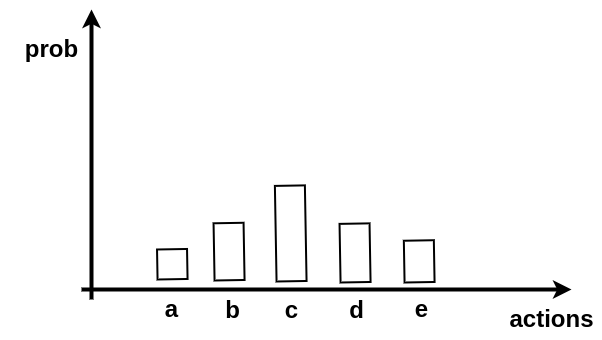
\includegraphics[width=.9\textwidth]{img/distribuicao.png}
	\end{center}
\end{frame}


\begin{frame}
	Se durante a experiência do agente, o mesmo percebe que uma ação tem \textit{reward} positivo (por exemplo, a ação \textit{c}) então...
	\begin{center}
		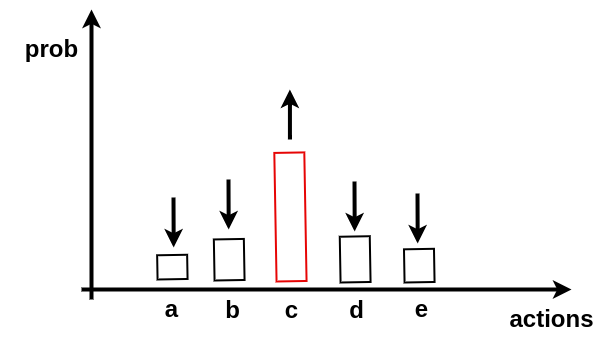
\includegraphics[width=.8\textwidth]{img/distribuicao_alterada.png}
	\end{center}
\end{frame}

\begin{frame}{Algoritmo}
	\begin{algorithmic} 
		\STATE \emph{\textbf{function} REINFORCE($\alpha$, $\gamma$, episódios):}
		\STATE inicializar os valores de $\theta$ para a policy $\pi(A|S,\theta)$ arbitrariamente
		\FOR {todos os episódios}
		\STATE gerar um episódio ${s_{0},a_{0},r_{1},\cdots,s_{T-1},a_{T-1},r_{T}}$ seguindo $\pi(.|.,\theta)$
		\FOR {cada passo dentro do episódio $t = 0, 1, 2, \cdots, T-1$}
			\STATE $G \leftarrow \sum_{k=t+1}^{T} \gamma^{k-t-1} \times r_{k}$
			\STATE $\theta \leftarrow \theta + \alpha \times \bigtriangledown \log \pi(a_{t}|s_{t}, \theta) \times G$
		\ENDFOR
		\ENDFOR
	\end{algorithmic}
\end{frame}

\begin{frame}
	\begin{algorithmic} 
		\STATE \emph{\textbf{function} REINFORCE($\alpha$, $\gamma$, episódios):}
		\STATE \HiLi inicializar os valores de $\theta$ para a policy $\pi(A|S,\theta)$ arbitrariamente
		\FOR {todos os episódios}
		\STATE gerar um episódio ${s_{0},a_{0},r_{1},\cdots,s_{T-1},a_{T-1},r_{T}}$ seguindo $\pi(.|.,\theta)$
		\FOR {cada passo dentro do episódio $t = 0, 1, 2, \cdots, T-1$}
		\STATE $G \leftarrow \sum_{k=t+1}^{T} \gamma^{k-t-1} \times r_{k}$
		\STATE $\theta \leftarrow \theta + \alpha \times \bigtriangledown \log \pi(a_{t}|s_{t}, \theta) \times G$
		\ENDFOR
		\ENDFOR
	\end{algorithmic}

	\begin{itemize}
		\item Inicializando uma rede neural
	\end{itemize}
\end{frame}


\begin{frame}
	\begin{algorithmic} 
		\STATE \emph{\textbf{function} REINFORCE($\alpha$, $\gamma$, episódios):}
		\STATE inicializar os valores de $\theta$ para a policy $\pi(A|S,\theta)$ arbitrariamente
		\FOR {todos os episódios}
		\STATE \HiLi gerar um episódio ${s_{0},a_{0},r_{1},\cdots,s_{T-1},a_{T-1},r_{T}}$ seguindo $\pi(.|.,\theta)$
		\FOR {cada passo dentro do episódio $t = 0, 1, 2, \cdots, T-1$}
		\STATE $G \leftarrow \sum_{k=t+1}^{T} \gamma^{k-t-1} \times r_{k}$
		\STATE $\theta \leftarrow \theta + \alpha \times \bigtriangledown \log \pi(a_{t}|s_{t}, \theta) \times G$
		\ENDFOR
		\ENDFOR
	\end{algorithmic}
	
	\begin{itemize}
		\item Executando um episódio por completo até encontrar um estado terminal ($T$).
		\item Armazena toda a sequência de ${s_{0},a_{0},r_{1},\cdots,s_{T-1},a_{T-1},r_{T}}$
	\end{itemize}
\end{frame}


\begin{frame}
	\begin{algorithmic} 
		\STATE \emph{\textbf{function} REINFORCE($\alpha$, $\gamma$, episódios):}
		\STATE inicializar os valores de $\theta$ para a policy $\pi(A|S,\theta)$ arbitrariamente
		\FOR {todos os episódios}
		\STATE gerar um episódio ${s_{0},a_{0},r_{1},\cdots,s_{T-1},a_{T-1},r_{T}}$ seguindo $\pi(.|.,\theta)$
		\FOR {cada passo dentro do episódio $t = 0, 1, 2, \cdots, T-1$}
		\STATE \HiLi $G \leftarrow \sum_{k=t+1}^{T} \gamma^{k-t-1} \times r_{k}$
		\STATE $\theta \leftarrow \theta + \alpha \times \bigtriangledown \log \pi(a_{t}|s_{t}, \theta) \times G$
		\ENDFOR
		\ENDFOR
	\end{algorithmic}
	
	\begin{itemize}
		\item Considerando $T=5$, temos:
		\begin{itemize}
			\item Para $a_{0}$ em $s_{0}$, $G = \gamma^{0}r_{1} + \gamma^{1}r_{2} + \gamma^{2}r_{3} + \gamma^{3}r_{4}$
			\item Para $a_{1}$ em $s_{1}$, $G = \gamma^{0}r_{2} + \gamma^{1}r_{3} + \gamma^{2}r_{4}$
		\end{itemize} 
		\item $G$ é chamado de \textit{discounted reward}.
	\end{itemize}
\end{frame}

\begin{frame}
	\begin{algorithmic} 
		\STATE \emph{\textbf{function} REINFORCE($\alpha$, $\gamma$, episódios):}
		\STATE inicializar os valores de $\theta$ para a policy $\pi(A|S,\theta)$ arbitrariamente
		\FOR {todos os episódios}
		\STATE gerar um episódio ${s_{0},a_{0},r_{1},\cdots,s_{T-1},a_{T-1},r_{T}}$ seguindo $\pi(.|.,\theta)$
		\FOR {cada passo dentro do episódio $t = 0, 1, 2, \cdots, T-1$}
		\STATE $G \leftarrow \sum_{k=t+1}^{T} \gamma^{k-t-1} \times r_{k}$
		\STATE \HiLi $\theta \leftarrow \theta + \alpha \times \bigtriangledown \log \pi(a_{t}|s_{t}, \theta) \times G$
		\ENDFOR
		\ENDFOR
	\end{algorithmic}
	
	\begin{itemize}
		\item $\pi(a_{t}|s_{t}, \theta)$ é a probabilidade de $a_{t}$ ser escolhida em $s_{t}$ seguindo $\pi(.|.,\theta)$
		\item a ideia principal desta equação é ajustar os pesos de $\theta$ usando um gradiente ascendente para aumentar a probabilidade de escolher trajetórias onde $G$ é alto.
		\item $\alpha$ é a taxa de aprendizado.  
	\end{itemize}
\end{frame}

\begin{frame}{Escolha de uma ação}
	\lstinputlisting[language=Python]{src/selectaction.py}
\end{frame}

\begin{frame}{Avaliação de uma ação}
	\lstinputlisting[language=Python]{src/evaluateaction.py}
\end{frame}

\begin{frame}{Definição da rede neural}
	\lstinputlisting[language=Python]{src/nn.py}
\end{frame}

\begin{frame}{Gerando os episódios}
	\small
	\lstinputlisting[language=Python]{src/trajetoria.py}
\end{frame}

\begin{frame}{Calculando $G$}
	\lstinputlisting[language=Python]{src/discountedrewards.py}
\end{frame}

\begin{frame}{Atualizando $\theta$}
	\scriptsize
	\lstinputlisting[language=Python]{src/theta.py}
\end{frame}

\begin{frame}{Usando o modelo}
	\lstinputlisting[language=Python]{src/usando.py}
\end{frame}

\begin{frame}{Treinando e salvando o modelo}
	\lstinputlisting[language=Python]{src/treinando.py}
\end{frame}

\begin{frame}{Lendo e usando o modelo}
	\lstinputlisting[language=Python]{src/lendo.py}
\end{frame}

\begin{frame}
	\begin{alertblock}{Sugestão de implementação}
		Implemente uma versão do algoritmo Reinforce com base no pseudo-código deste material e com base nos trechos de códigos disponibilizados. 
	\end{alertblock}

	\begin{alertblock}{Ambientes}
	Teste nos ambientes CartPole-v1 e LunarLander-v2. 
	\end{alertblock}
\end{frame}
			
\begin{frame}{Referências}
	\begin{itemize}
		\item Williams, R.J. Simple statistical gradient-following algorithms for connectionist reinforcement learning. Machine Learning 8, 229–256 (1992). https://doi.org/10.1007/BF00992696
	\end{itemize}
\end{frame}
		
\end{document}
	
